\documentclass[a4paper, 12pt]{article}
\usepackage{geometry}
\geometry{a4paper,
total={170mm,257mm},left=2cm,right=2cm,
top=2cm,bottom=2cm}

\usepackage{calc}
\usepackage{setspace}
\usepackage{indentfirst}

\usepackage{subfigure}
\usepackage[table,xcdraw]{xcolor}
\usepackage{mathtext}
\usepackage{wrapfig}
\usepackage{amsmath}
\usepackage[T2A]{fontenc}
\usepackage[utf8]{inputenc}
\usepackage[english,russian]{babel}
\usepackage{graphicx, float}
\usepackage{tabularx, colortbl}
\usepackage{caption}
\captionsetup{labelsep=period}

\newcommand{\parag}[1]{\paragraph*{#1:}}
\DeclareSymbolFont{T2Aletters}{T2A}{cmr}{m}{it}
\newcounter{Points}
\setcounter{Points}{1}
\newcommand{\point}{\arabic{Points}. \addtocounter{Points}{1}}
% \newcolumntype{C}{>{\centering\arraybackslash}X}

\author{Калинин Даниил, Б01-110}
\date{1 мая 2022 г.}
\title{Лабораторная работа 2.3.1. Получение и измерение вакуума.}

\begin{document}
\maketitle

\parag {Цель работы}
\begin{enumerate}
    \item измерение объемов форвакуумной и высоковакуумной частей установки;
    \item определение скорости откачки системы в стационарном режиме, а также по ухудшению и улучшению вакуума. 
\end{enumerate}

\parag {В работе используются}
вакуумная установка с манометрами: масляным, термопарным и ионизационным.

\parag {Экспериментальная установка}~\\
В данной работе используются традиционные методы откачки механическим форвакуумным насосом до давления $10^{-2}$ торр и диффузионным масляным насосом до давления $10^{-4}$ торр. \\
Установка изготовлена из стекла,
и состоит из форвакуумного баллона (ФБ), высоковакуумного диффузионного насоса (ВН), высоковакуумного баллона (ВБ), масляного (М) и ионизационного (И) манометров, термопарных манометров ($\text{М}_1$ и $\text{М}_2$), форвакуумного насоса (ФН) и соединительных кранов ($K_1, K_2,..., K_6$) (рис. 1). Кроме того, в состав установки входят: вариатор
(автотрансформатор с регулируемым выходным напряжением), или
реостат и амперметр для регулирования тока нагревателя диффузионного насоса. \\
\begin{figure}[!h]
\centering
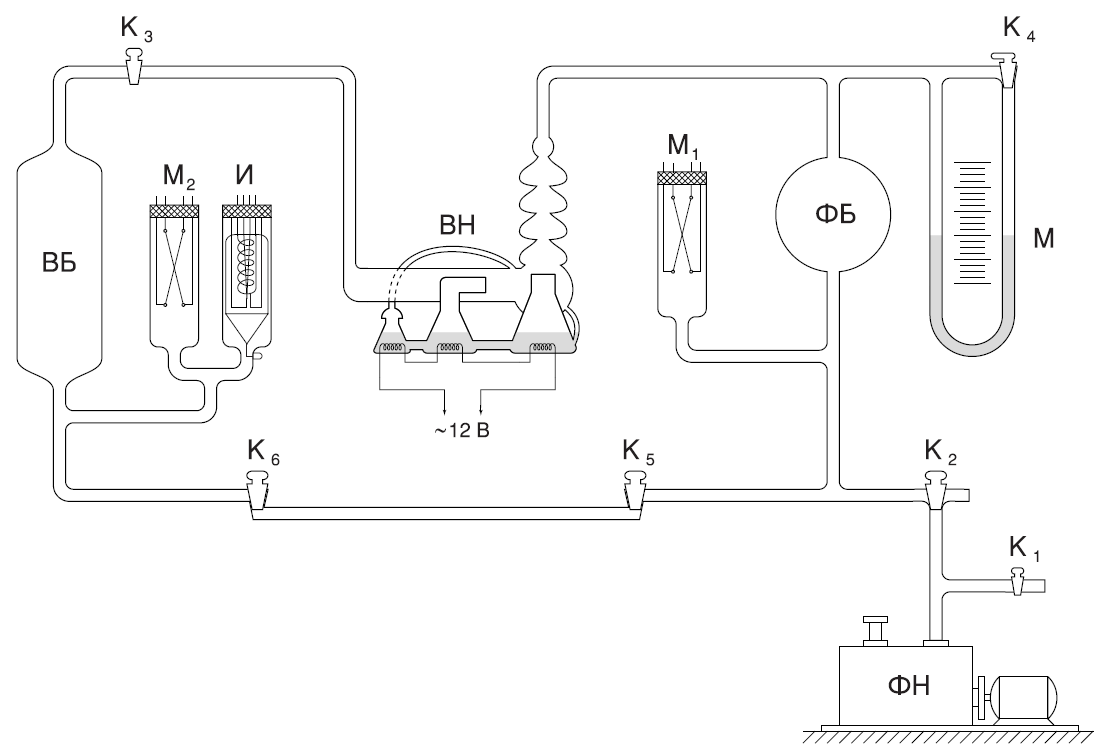
\includegraphics[width=0.5\linewidth]{setup.png}
\caption[]{Схема установки}
\label{fig:Схема установки}
\end{figure}
Все краны вакуумной установки стеклянные. Стенки кранов тонкие, пробки кранов полые и составляют одно целое с рукоятками. Пробки кранов притерты к корпусам. Для герметизации используется вакуумная смазка. \\
Устройство и принцип действия \textit{форвакуумного насоса} схематически, но довольно ясно изображены на рис 2. В положениях <<а>> и <<б>> пластина <<А>> засасывает разреженный воздух из откачиваемого объёма, а пластина <<Б>> вытесняет ранее захваченный воздух в атмосферу. В положениях <<в>> и <<г>> пластины поменялись ролями.
\begin{figure}[!h]
\centering
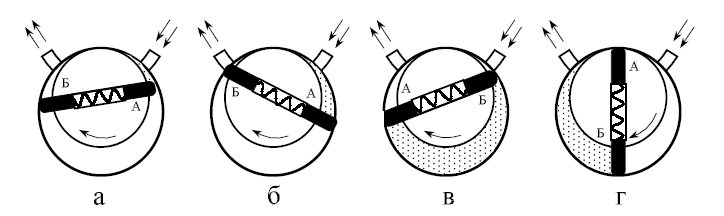
\includegraphics[width=0.9\linewidth]{forvakuum.png}
\caption[]{Схема действия ротационного двухпластинчатого форвакуумного насоса}
\label{fig:Схема ФВ насоса}
\end{figure}
Устройство и принцип действия \textit{диффузионного насоса} схематически изображены на рис 2. Такой насос работает в тысячи раз быстрее форвакуумного. Его действие основано на диффузии. Масло, налитое в сосуд А, подогревается электрической печкой. Пары масла поднимаются по трубке Б и вырываются из сопла В. Струя паров увлекает молекулы газа, которые поступают из откачиваемого сосуда через трубку ВВ. В трубке Г мало осаждается и стекает вниз. Оставшийся газ, выходя в трубку ФВ, откачивается форвакуумным насосом. \\
Диффузионный насос работает наиболее эффективно, когда длина свободного пробега молекул примерно равна ширине кольцевого зазора между соплом В и стенками трубки ВВ. Давление насыщенных паров масла при рабочей температуре, создаваемой обогревателем сосуда А, много больше $5\cdot 10^{-2}$ торр, поэтому пары масла создают плотную струю, увлекающую с собой молекулы газа.
\begin{figure}[!h]
\centering
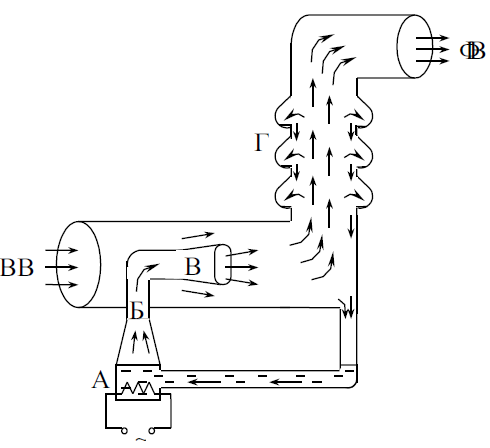
\includegraphics[width=0.4\linewidth]{highvakuum.png}
\caption[]{Схема работы диффузионного насоса}
\label{fig:Схема ВВ насоса}
\end{figure}
Диффузионный насос, используемый в нашей установке (см. рис 1) имеет две ступени и соответственно два сопла. Одно сопло вертикальное (первая ступень), второе горизонтальное (вторая ступень). За второй ступенью имеется ещё одна печь, но пар из этой печи поступает не в сопло, а по тонкой трубке подводится ближе к печке первой ступени. Эта печь осуществляет фракционирование масла. Легколетучие фракции масла, испаряясь, поступают в первую ступень, обогащая её. По этой причине плотность струи первой ступени выше, и эта ступень начинает откачивать при более высоком давлении в форвакуумной части. Вторая ступень обогащается малолетучими фракциями масла. Плотность струи второй ступени меньше, но меньше и давление насыщенных паров. Соответственно, в откачиваемый объем поступает меньше паров масла, и его удаётся откачать до более высокого вакуума.  \\


\parag {Теоритическая справка} ~\\
\textbf{Процесс откачки}\\
Опишем процесс откачки математически: 
Пусть W --- объем газа, удаляемого из сосуда при данном давлении за единицу времени, $Q_i$ для различных значений i обозначим различные притоки газа в сосуд (в единицах PV), такие как течи извне $Q_\text{и}$, десорбция с поверхностей внутри сосуда $Q_\text{д}$, обратный ток через насос $Q_\text{н}$. Тогда, приравнивая убыль газа из сосуда (с точностью до $RT/\mu$) в единицу времени $-VdP$ и сумму перечисленных токов? имеем:
 \begin{equation}
 	-VdP = (PW - \sum_i Q_i)dt
 \end{equation}
 При достижении предельного вакуума устанавливается давление $P_{\text{пр}}$, и $dP = 0$. Тогда
 \begin{equation}
 	 W = ( \sum_i Q_i )/P_{\text{пр}}
 \end{equation}
 Поскольку обычно $Q_\text{и}$ постоянно, а $Q_\text{н}$ и $Q_\text{д}$ слабо зависят от времени, также считая постоянной W, можем проинтегрировать (1) и получить:
 \begin{equation}
 	P - P_{\text{пр}} = (P_0 - P_{\text{пр}})\exp(-\frac{W}{V}t)
 \end{equation}
Полная скорость откачки $W$, собственная скорость откачки насоса $W_{\text{н}}$ и проводимости элементов системы $C_1, C_2,...$ соотносятся согласно формуле (4), и это учтено в конструкции установки.
 \begin{equation}
 \frac{1}{W} = \frac{1}{W} + \frac{1}{C_1} + \frac{1}{C_2} + ...
\end{equation}

\textbf{Течение газа через трубу}\\
Характер течения газа существенно зависит от соотношения между размерами системы и длиной свободного пробега молекул. При атмосферном и форвакуумном давлениях  длина свободного пробега меньше диаметра трубок, и течение газа определяется его вязкостью, т.е. взаимодействием молекул. При высоком вакууме течение существеннее определяется взаимодействием со стенками \\
Для количества газа, протекающего через трубу длины $l$ и радиуса $r$ в условиях высокого вакуума, справедлива формула:
\begin{equation}
	\frac{d(PV)}{dt} = \frac{4}{3}r^3\sqrt{\frac{2\pi RT}{\mu}}\frac{P_2 - P_1}{l}
\end{equation}
Если труба соединяет насос установку, то давлением $P_1$ у насоса можно пренебречь. Давление в сосуде $P = P_2$. Тогда имеем:
\begin{equation}
C_\text{тр} = \left(\frac{dV}{dt}\right)_\text{тр} = \frac{4r^3}{3l}\sqrt{\frac{2\pi RT}{\mu}}
\end{equation}
Для пропускной способности отверстий имеется формула
\begin{equation}
C_\text{отв} = \left(\frac{dV}{dt}\right)_\text{отв} = S\frac{\bar{\upsilon}}{4}
\end{equation}
Для воздуха при комнатной температуре $\bar{\upsilon}/4 = 110~\text{м/с} = 11~\text{л/c}\cdot\text{см}^2$.

\parag {Ход работы} ~\\

\point \textbf{Измерение объёмов форвакуумной и высоковакуумной частей установки}
	\begin{enumerate}
		\item Проверяем, что $K_4$ открыт, впускаем в установку атмосферный воздух через краны $K_1$ и $K_2$. <<Запираем>> в капилляре атмосферный воздух кранами $K_5$ и $K_6$. Объем капилляра в используемой установке: $$V_\text{к} = 50~ \text{см}^3.$$
		\item Закрываем $K_1$ и $K_2$, включаем форвакуумный насос и даём ему откачать себя. Подключаем установку к насосу краном $K_2$. Откачиваем установку до $10^{-2}$ торр. Отсоединяем установку краном $K_2$, и оставляем насос работать <<на себя>>. Перекрываем  $K_3$, отделяя высоковакуумною часть установки. Закрываем  $K_4$, чтобы привести в готовность масляный манометр.
		\item Открываем  $K_5$, чтобы <<запертый>> ранее воздух заполнил форвакуумную часть установки, снимаем давление с помощью вакуумного манометра, измерив разность высот столбиков масла (приводим результаты и повторного измерения):
		$$
		\Delta h_1 = (15.1\pm0.1) ~\text{мм};\quad \Delta h_2 (15.2\pm0.1) ~\text{мм}
		$$
		Погрешность измерения величин определяется ценой деления шкалы манометра и способностью разглядеть показания.
		\item Имея в виду, что плотность масла в манометре равна 885 г/л, и считая, что установившееся давление много больше форвакуумного, получаем:
		$$
		P_1 = (1.31\pm0.01)~\text{Па};\quad P_2 = (1.32\pm0.01)~\text{Па}
		$$
		Пользуясь законом Бойля-Мариотта (т.к. расширение газа изотермическое), используя среднее значение измеренного давления, получаем
		$$
		V_\text{ФВ} = (3750\pm20)~\text{см}^3
		$$
		\item Аналогично, открыв кран $K_3$, получив значения разности высот на манометре
		$$
		\Delta h_1 = (10.3\pm0.1) \text{мм}; \Delta h_2 (10.3\pm0.1) \text{мм},
		$$
		Получаем объем высоковакуумной части установки, вычтя из полученного законом Бойля-Мариотта объёма двух частей установки объем измеренной ранее части (погрешности складываются):
		$$
		V_\text{ВВ} = (1760\pm60)~\text{см}^3
		$$
		\item Открываем кран $K_4$.
	\end{enumerate}

\point  \textbf{Получение высокого вакуума}
	\begin{enumerate}
	\item Откачиваем установку ФВ насосом.
	\item Включаем термопарные манометры и определяем давление в установке по градуировочной кривой.
	\item По достижении форвакуума закрываем $K_5$ и начинаем откачку высоковакуумного баллона с помощью диффузионного насоса.
	\item Включаем ионизационную лампу.
	\item Измеряем давление с помощью микроамперметра.
	
	$$P_{\text{пр}} = 1,1\cdot10^{-4} ~\text{торр}$$	
\end{enumerate}

\point \textbf{Измерение скорости по ухудшению и улучшению вакуума}
\begin{enumerate}
	\item Закрываем кран $K_3$, отключая тем самым откачку вакуума и записываем изменения показаний микроамперметра, пока вакуум не ухудшится до $6\cdot10^{-4}$ торр. Затем открываем $K_3$ и так же записываем улучшение вакуума. Приводим результаты повторных измерений в таблице 1 и на графиках (рис. 7 и 8).
	\begin{table}[!h]
		\centering
		\resizebox{0.9\textwidth}{!}{%
			\begin{tabular}{|c|l|cl|c|c|c|c|cc}
				\hline
				\multicolumn{2}{|c|}{{\color[HTML]{000000} \textbf{Улучшение,   1}}} & \multicolumn{2}{c|}{{\color[HTML]{000000} \textbf{Улучшение, 2}}} & \multicolumn{2}{c|}{{\color[HTML]{000000} \textbf{Ухудшение, 1}}} & \multicolumn{2}{c|}{{\color[HTML]{000000} \textbf{Ухудшение, 2}}} & \multicolumn{2}{c|}{{\color[HTML]{000000} \textbf{Ухудшение, 3}}} \\ \hline
				{\color[HTML]{000000} \textbf{t, с}} & \multicolumn{1}{c|}{{\color[HTML]{000000} \textbf{p, торр}}} & \multicolumn{1}{l|}{{\color[HTML]{000000} \textbf{t, с}}} & {\color[HTML]{000000} \textbf{p, торр}} & \multicolumn{1}{l|}{{\color[HTML]{000000} \textbf{t, с}}} & {\color[HTML]{000000} \textbf{p, торр}} & \multicolumn{1}{l|}{{\color[HTML]{000000} \textbf{t, с}}} & \multicolumn{1}{l|}{{\color[HTML]{000000} \textbf{p, торр}}} & \multicolumn{1}{l|}{{\color[HTML]{000000} \textbf{t, с}}} & \multicolumn{1}{l|}{{\color[HTML]{000000} \textbf{p, торр}}} \\ \hline
				{\color[HTML]{000000} 0} & {\color[HTML]{000000} 0,0006} & \multicolumn{1}{c|}{{\color[HTML]{000000} 0}} & {\color[HTML]{000000} 0,000615} & {\color[HTML]{000000} 0} & {\color[HTML]{000000} 0,00009} & {\color[HTML]{000000} 0} & {\color[HTML]{000000} 0,00008} & \multicolumn{1}{c|}{{\color[HTML]{000000} 0}} & \multicolumn{1}{c|}{{\color[HTML]{000000} 0,0001}} \\ \hline
				{\color[HTML]{000000} 0,167} & {\color[HTML]{000000} 0,00058} & \multicolumn{1}{c|}{{\color[HTML]{000000} 0,33}} & {\color[HTML]{000000} 0,0006} & {\color[HTML]{000000} 5,5} & {\color[HTML]{000000} 0,00012} & {\color[HTML]{000000} 4} & {\color[HTML]{000000} 0,00012} & \multicolumn{1}{c|}{{\color[HTML]{000000} 5}} & \multicolumn{1}{c|}{{\color[HTML]{000000} 0,00015}} \\ \hline
				{\color[HTML]{000000} 0,33} & {\color[HTML]{000000} 0,000555} & \multicolumn{1}{c|}{{\color[HTML]{000000} 0,9}} & {\color[HTML]{000000} 0,00056} & {\color[HTML]{000000} 10} & {\color[HTML]{000000} 0,00016} & {\color[HTML]{000000} 12} & {\color[HTML]{000000} 0,00018} & \multicolumn{1}{c|}{{\color[HTML]{000000} 12}} & \multicolumn{1}{c|}{{\color[HTML]{000000} 0,0002}} \\ \hline
				{\color[HTML]{000000} 0,5} & {\color[HTML]{000000} 0,00054} & \multicolumn{1}{c|}{{\color[HTML]{000000} 1,5}} & {\color[HTML]{000000} 0,00052} & {\color[HTML]{000000} 16} & {\color[HTML]{000000} 0,0002} & {\color[HTML]{000000} 20} & {\color[HTML]{000000} 0,00024} & \multicolumn{1}{c|}{{\color[HTML]{000000} 18}} & \multicolumn{1}{c|}{{\color[HTML]{000000} 0,00025}} \\ \hline
				{\color[HTML]{000000} 0,75} & {\color[HTML]{000000} 0,00052} & \multicolumn{1}{c|}{{\color[HTML]{000000} 2}} & {\color[HTML]{000000} 0,00046} & {\color[HTML]{000000} 21} & {\color[HTML]{000000} 0,00024} & {\color[HTML]{000000} 26} & {\color[HTML]{000000} 0,00028} & \multicolumn{1}{c|}{{\color[HTML]{000000} 25}} & \multicolumn{1}{c|}{{\color[HTML]{000000} 0,0003}} \\ \hline
				{\color[HTML]{000000} 1} & {\color[HTML]{000000} 0,0005} & \multicolumn{1}{c|}{{\color[HTML]{000000} 2,4}} & {\color[HTML]{000000} 0,00042} & {\color[HTML]{000000} 26} & {\color[HTML]{000000} 0,00028} & {\color[HTML]{000000} 31} & {\color[HTML]{000000} 0,00032} & \multicolumn{1}{c|}{{\color[HTML]{000000} 32}} & \multicolumn{1}{c|}{{\color[HTML]{000000} 0,00035}} \\ \hline
				{\color[HTML]{000000} 1,25} & {\color[HTML]{000000} 0,00047} & \multicolumn{1}{c|}{{\color[HTML]{000000} 3}} & {\color[HTML]{000000} 0,00038} & {\color[HTML]{000000} 32} & {\color[HTML]{000000} 0,00032} & {\color[HTML]{000000} 37} & {\color[HTML]{000000} 0,00036} & \multicolumn{1}{c|}{{\color[HTML]{000000} 39}} & \multicolumn{1}{c|}{{\color[HTML]{000000} 0,0004}} \\ \hline
				{\color[HTML]{000000} 1,5} & {\color[HTML]{000000} 0,00043} & \multicolumn{1}{c|}{{\color[HTML]{000000} 4}} & {\color[HTML]{000000} 0,00032} & {\color[HTML]{000000} 40} & {\color[HTML]{000000} 0,00038} & {\color[HTML]{000000} 43} & {\color[HTML]{000000} 0,0004} & \multicolumn{1}{c|}{{\color[HTML]{000000} 46}} & \multicolumn{1}{c|}{{\color[HTML]{000000} 0,00045}} \\ \hline
				{\color[HTML]{000000} 2} & {\color[HTML]{000000} 0,0004} & \multicolumn{1}{c|}{{\color[HTML]{000000} 5}} & {\color[HTML]{000000} 0,00028} & {\color[HTML]{000000} 47} & {\color[HTML]{000000} 0,00042} & {\color[HTML]{000000} 49} & {\color[HTML]{000000} 0,00044} & \multicolumn{1}{c|}{{\color[HTML]{000000} 52}} & \multicolumn{1}{c|}{{\color[HTML]{000000} 0,0005}} \\ \hline
				{\color[HTML]{000000} 3} & {\color[HTML]{000000} 0,00032} & \multicolumn{1}{c|}{{\color[HTML]{000000} 6}} & {\color[HTML]{000000} 0,00024} & {\color[HTML]{000000} 52} & {\color[HTML]{000000} 0,00046} & {\color[HTML]{000000} 54} & {\color[HTML]{000000} 0,00048} & \multicolumn{1}{c|}{{\color[HTML]{000000} 60}} & \multicolumn{1}{c|}{{\color[HTML]{000000} 0,00055}} \\ \hline
				{\color[HTML]{000000} 4} & {\color[HTML]{000000} 0,00027} & \multicolumn{1}{c|}{{\color[HTML]{000000} 8}} & {\color[HTML]{000000} 0,00019} & {\color[HTML]{000000} 57} & {\color[HTML]{000000} 0,0005} & {\color[HTML]{000000} 60} & {\color[HTML]{000000} 0,00052} & \multicolumn{1}{c|}{{\color[HTML]{000000} 68}} & \multicolumn{1}{c|}{{\color[HTML]{000000} 0,0006}} \\ \hline
				{\color[HTML]{000000} 6} & {\color[HTML]{000000} 0,0002} & \multicolumn{1}{c|}{{\color[HTML]{000000} 12}} & {\color[HTML]{000000} 0,00014} & {\color[HTML]{000000} 66} & {\color[HTML]{000000} 0,00055} & {\color[HTML]{000000} 68} & {\color[HTML]{000000} 0,00056} & {\color[HTML]{000000} } & {\color[HTML]{000000} } \\ \cline{1-8}
				{\color[HTML]{000000} 9} & {\color[HTML]{000000} 0,00015} & {\color[HTML]{000000} } & {\color[HTML]{000000} } & {\color[HTML]{000000} 74} & {\color[HTML]{000000} 0,0006} & {\color[HTML]{000000} 74} & {\color[HTML]{000000} 0,0006} & {\color[HTML]{000000} } & {\color[HTML]{000000} } \\ \cline{1-2} \cline{5-8}
			\end{tabular}%
		}
	\caption{Зависимости давления от времени}	
	\end{table}

	\begin{figure}[!h]
		\begin{center}
			\subfigure[Измерение 1]{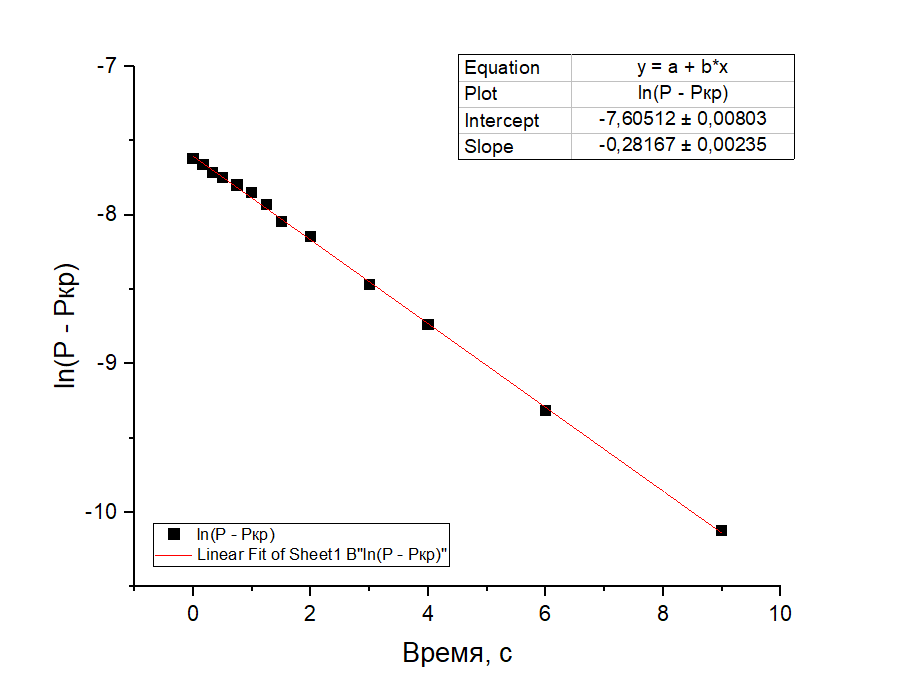
\includegraphics[width=0.45\textwidth]{eksp1.png}}
			\subfigure[Измерение 2]{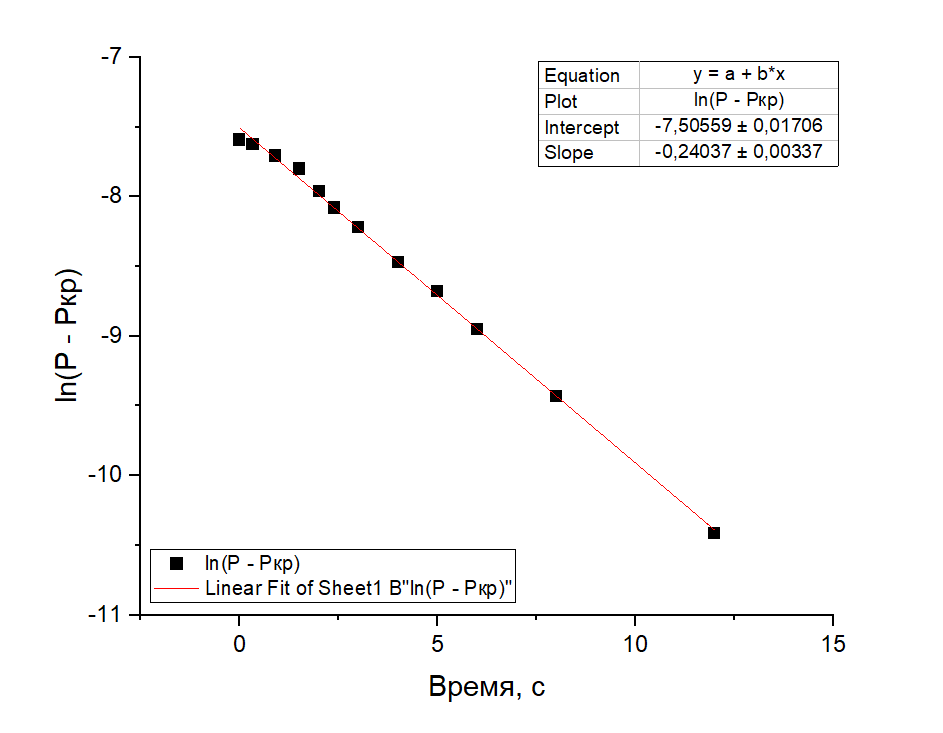
\includegraphics[width=0.45\textwidth]{eksp2.png}}
		\end{center}
		\caption{Зависимость давления от времени по улучшении вакуума}
	\end{figure}

	\begin{figure}[!h]
		\begin{center}
			\subfigure[Измерение 1]{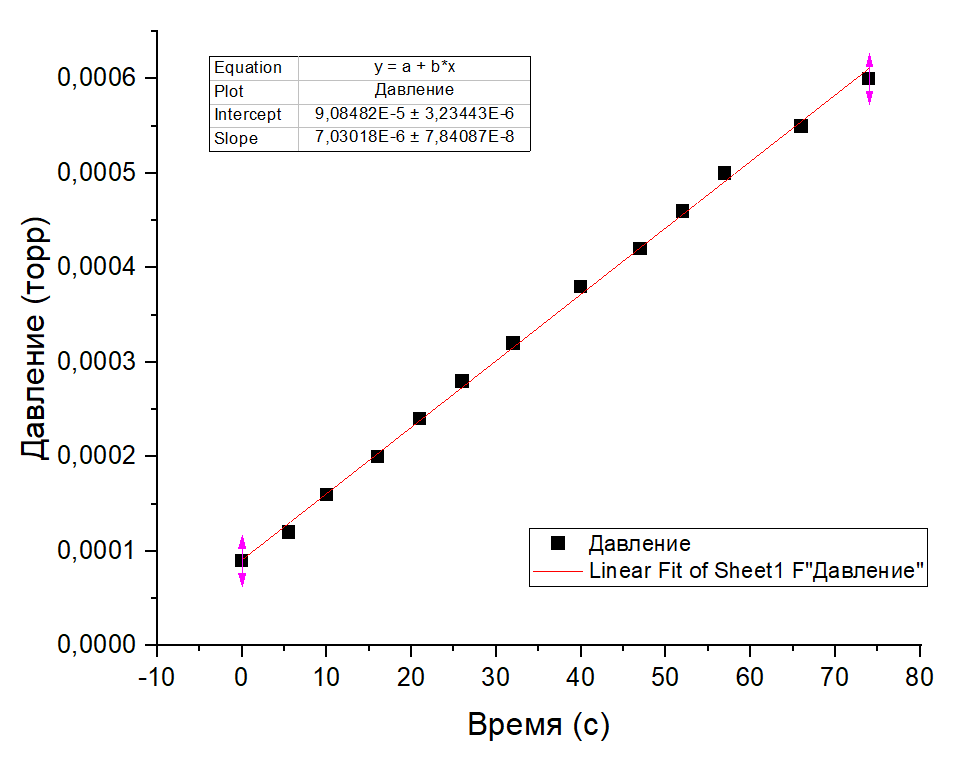
\includegraphics[width=0.3\textwidth]{line_1.png}}
			\subfigure[Измерение 2]{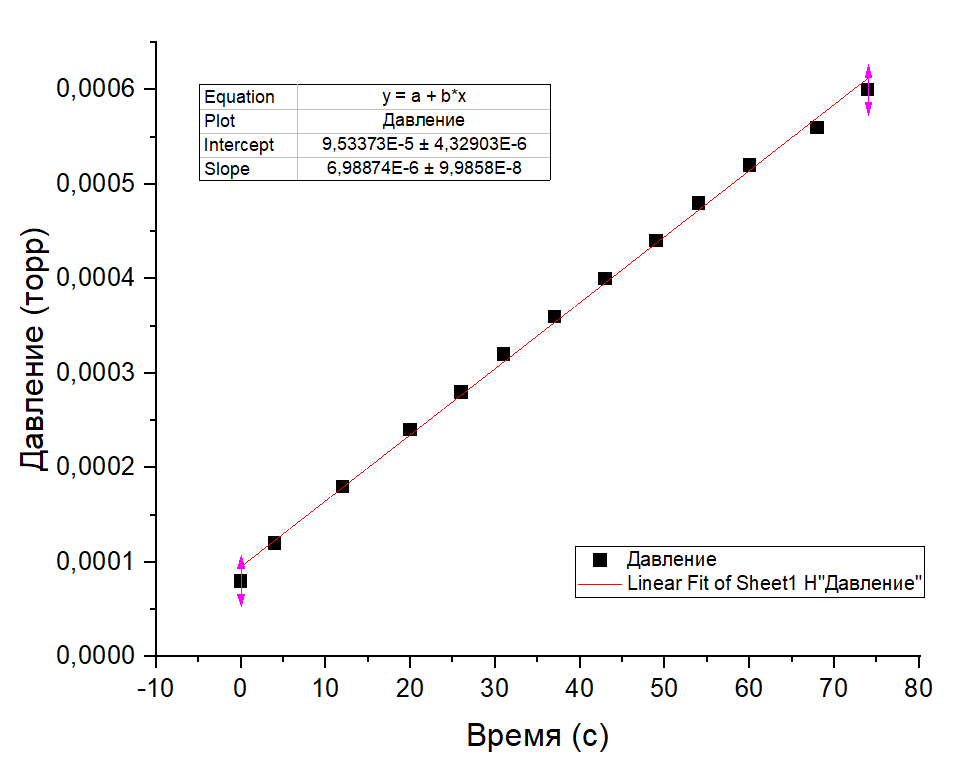
\includegraphics[width=0.3\textwidth]{line_2.png}}
			\subfigure[Измерение 3]{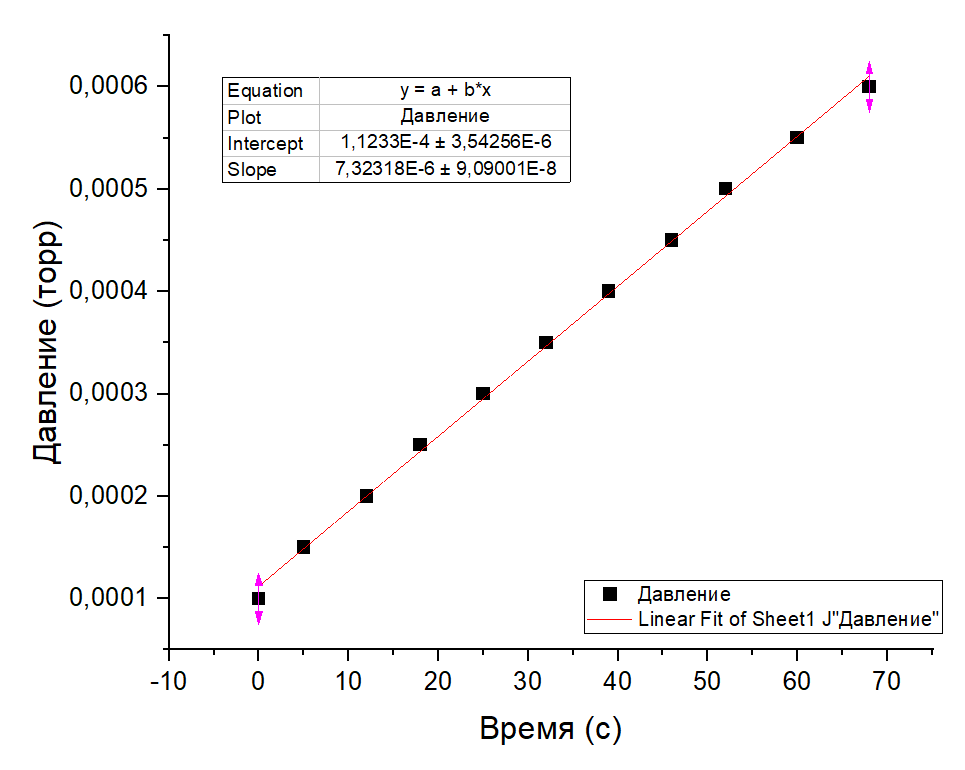
\includegraphics[width=0.3\textwidth]{line_3.png}}
		\end{center}
		\caption{Зависимость давления от времени по улучшении вакуума}
	\end{figure}
	\item
	Рассчитав коэффициенты наклона графиков 7(а) и 7(б) и зная объем высоковакуумной части установки, получим скорость откачки W диффузионного насоса, сравнив графики с зависимостью (4). Считаем $$W = -\bar{a}\cdot V, \quad\varepsilon_W^2 = \varepsilon_{\bar{a}}^2 + \varepsilon_V^2$$,  где $\bar{a}$ --- среднее коэффициентов наклона из зависимостей 7(а) и 7(б). Имеем:
	$$W = (0,461\pm0,016) ~\text{л/с}$$
	\item
	Имея в виду соотношения (1) для случая ухудшения вакуума (без откачки), оценим $Q_\text{н}$ c помощью полученных зависимостей 8(а, б, в). Считаем $$\frac{dP}{dt} = \bar{a}$$ где $\bar{a}$ --- среднее коэффициентов наклона из зависимостей 8(а), 8(б), 8(в). Имеем:
	$$Q_\text{н} + Q_\text{д} = (1,26\pm0,04)\cdot 10^{-5} ~\text{торр}\cdot\text{л/c}~(\varepsilon = 0,03)$$, 

\end{enumerate}

\parag {Заключение} ~\\
\begin{enumerate}
	\item В ходе данной работы была проверена методика по измерению производительности высоковакуумного насоса.
	\item С хорошей точностью была измерена производетельность диффузионного насоса.
\end{enumerate}
\end{document}
